\documentclass{article}

\usepackage[utf8]{inputenc}
\usepackage[T1]{fontenc}
\usepackage{lipsum}
\usepackage{graphicx}
\usepackage{amsmath}
\usepackage[margin=1in]{geometry}
\usepackage{titlesec}
\usepackage{enumitem}

\titleformat{\section} 
{\LARGE\bfseries}{\thesection}{1em}{}

\titleformat{\subsection} 
{\Large\bfseries}{\thesection}{1em}{}

\begin{document}

\pagestyle{empty}

\section*{Progettazione logica} 
\large

L'obiettivo della \textbf{progettazione logica} è la realizzazione del modello logico a partire dalle informazioni del modello E/R. Una possibilità è quella di tradurre ogni entità ed ogni relazione del modello E/R con una tabella corrispondente. Questo procedimento è assolutamente da evitare per due problematiche principali.\\
La prima problematica risale nell'\textbf{efficienza}, ovvero il numero di tabelle generate, o l'efficienza delle operazioni sui dati.\\
La seconda problematica invece è la \textbf{correttezza}, ovvero come si possono tradurre le generalizzazioni o altre strutture senza equivalenti nel modello E/R.\vspace*{14pt}\\
Per garantire la qualità dello schema prodotto, la \textbf{progettazione logica} tipicamente include due passaggi:
\begin{itemize}[label={-}, leftmargin=1cm]
    \itemsep0em
    \item \textbf{Ristrutturazione del modello concettuale}: modificare lo schema E/R al fine di abilitare la traduzione nel modello logico e di ottimizzare il progetto nel suo complesso
    \item \textbf{Traduzione nel modello logico}: traduzione dei costrutti del modello E/R nei costrutti equivalenti del modello relazionale
\end{itemize}

\subsection*{Ristrutturazione del modello concettuale}
\large

Prima di tradurre il modello E/R, è necessario \textbf{ristrutturarlo} per motivi di \textbf{correttezza ed efficienza}. Sono presenti quindi delle \textit{fasi}, alcune delle quali potrebbero non essere necessarie.\vspace*{14pt}\\
\textit{Eliminazione delle generalizzazioni}\\
Per \textbf{eliminare le generalizzazioni} sono presenti \textit{tre} soluzioni principali:
\begin{itemize}[label={-}, leftmargin=1cm]
    \itemsep0em
    \item \textbf{Soluzione 1}: accorpamento delle entità figlie nell'entità genitore, con accorpamento dei relativi attributi e delle relazioni
    \begin{center}
        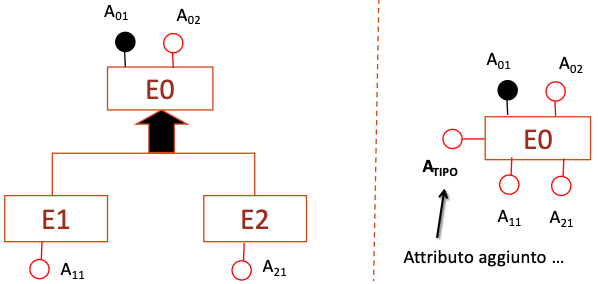
\includegraphics[width=0.5\textwidth]{foto 1.png}
    \end{center}
    Questa soluzione introduce valori nulli ed un attributo aggiuntivo, ma è \textbf{conveniente quando non ci sono troppe differenze concettuali} tra E0, E1 ed E2
    \item \textbf{Soluzione 2}: accorpamento delle entità genitore nelle entità figlie, con accorpamento dei relativi attributi e delle relazioni
    \begin{center}
        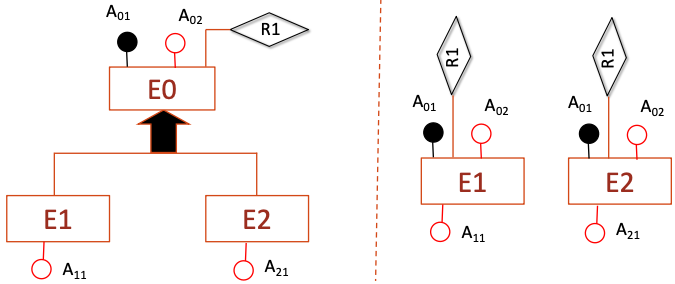
\includegraphics[width=0.5\textwidth]{foto 2.png}
    \end{center}
    Questa soluzione è \textbf{possibile solo se la generalizzazione è totale}, non introduce valori nulli, ma è \textbf{conveniente quando ci sono operazioni che coinvolgono per lo più E1 ed E2 ma non l'entità genitore E0}
    \item \textbf{Soluzione 3}: sostituzione delle generalizzazioni con relazioni tra entità genitore ed entità figlie
    \begin{center}
        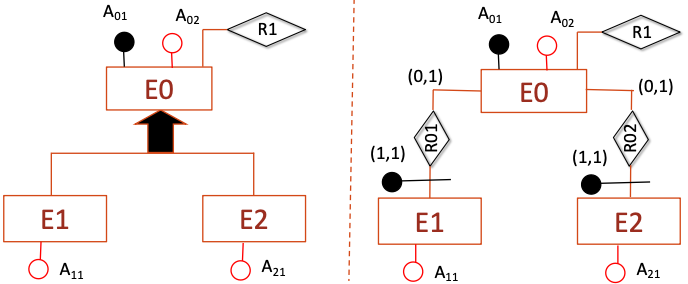
\includegraphics[width=0.5\textwidth]{foto 3.png}
    \end{center}
    Questa soluzione non introduce valori nulli, ed è \textbf{utile quando ci sono operazioni che si riferiscono solo ad istanze di E1, E2 ed E0}, ma presenta la necessità di introdurre dei vincoli: il primo impone che un'occorrenza di E0 \textbf{non può partecipare in contemporanea} ad R01 ed R02; il secondo impone che la \textbf{generalizzazione sia totale}, quindi ogni occorrenza di E0 deve appartenere ad R01 o R02\\
\end{itemize}
Si osservi un esempio di eliminazione delle generalizzazioni:
\begin{center}
    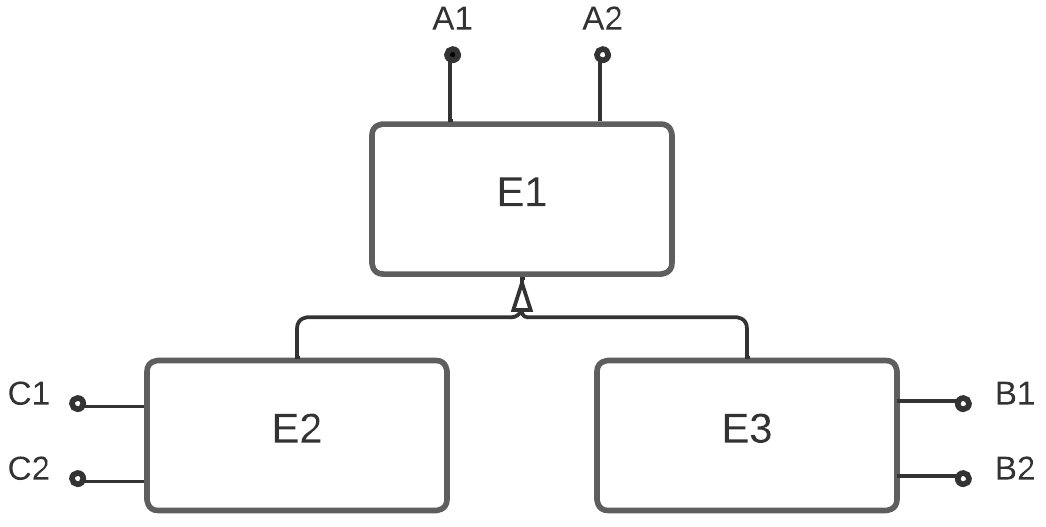
\includegraphics[width=0.5\textwidth]{esempio1.png}
\end{center}
Sono presenti 30 istanze di \textit{E1} (non sono ne \textit{E2} ne \textit{E3}), 20 istanze di \textit{E2}, 10 istanze di \textit{E3}. Si osservino le possibili soluzioni:\vspace{90pt}\\
\textit{Soluzione 1}
\begin{center}
    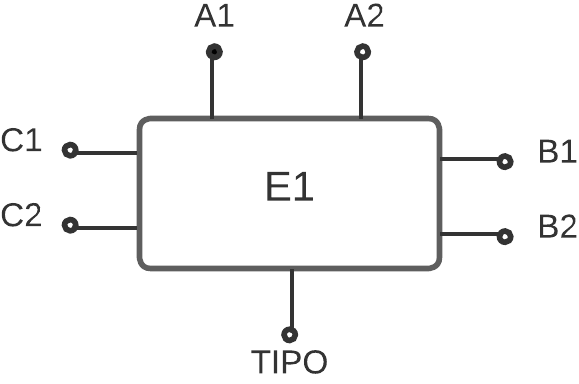
\includegraphics[width=0.4\textwidth]{esempio2.png}
\end{center}
Il numero di campi nulli è \textit{(10 $\cdot$ 2) + (20 $\cdot$ 2) + (30 $\cdot$ 4) = 180 NULL}\vspace{14pt}\\
\textit{Soluzione 2}\\
\textbf{Non è possibile}, la generalizzazione \textbf{non è totale}!\vspace*{14pt}\\
\textit{Soluzione 3}
\begin{center}
    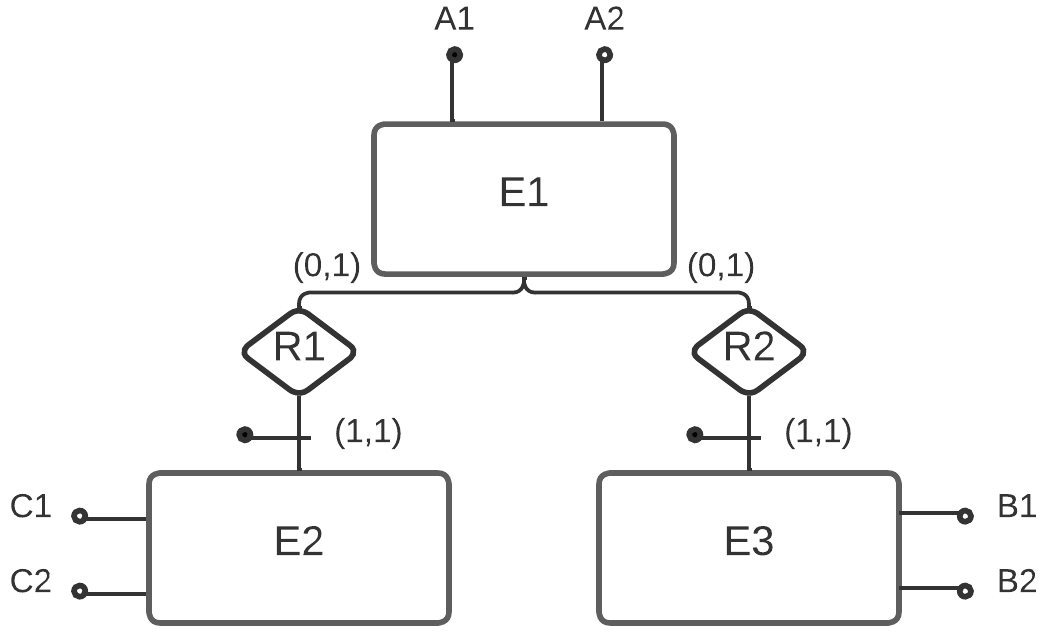
\includegraphics[width=0.5\textwidth]{esempio3.png}
\end{center}
Il numero di campi nulli in questo caso è 0.\vspace{14pt}\\
\textit{Eliminazione degli attributi multi-valore}\\
Gli \textbf{attributi multivalore} non sono presenti nel modello logico, ma possono essere modellati anche con una \textbf{relazione uno a molti}.
\begin{center}
    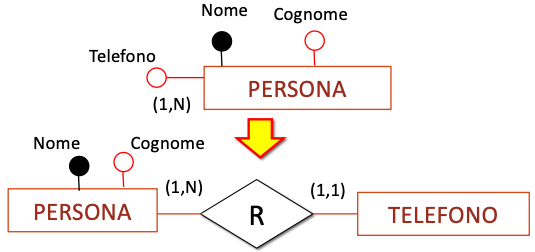
\includegraphics[width=0.5\textwidth]{foto 4.png}
\end{center}
Questa soluzione non introduce valori NULL, ma \textbf{aumenta il numero di entità} presenti nel sistema.\vspace{70pt}\\
\textit{Partizionamento/accorpamento di concetti (fase opzionale)}\\
Per un dato modello E/R, è possibile \textbf{ridurre il numero di accessi}:
\begin{itemize}[label={-}, leftmargin=1cm]
    \itemsep0em
    \item Separando attributi che vengono acceduti separatamente, attraverso \textbf{partizionamenti}
    \item Raggruppando attributi di entità diverse ma acceduti allo stesso tempo, attraverso \textbf{accorpamenti}
    \item Avendo una \textbf{stima sul volume dei dati} per un'indicazione se(come) partizionare(accorpare) entità\\
\end{itemize}
Gli \textbf{accorpamenti di entità} riguardano \textbf{relazioni uno ad uno}. Possono essere eseguiti nel seguente modo:
\begin{center}
    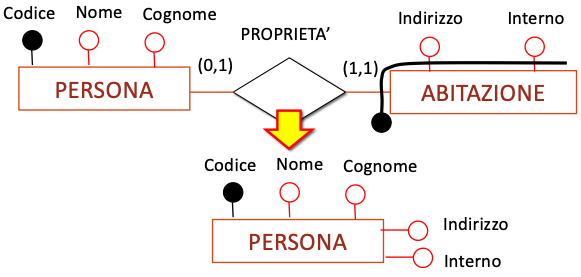
\includegraphics[width=0.5\textwidth]{foto 5.png}
\end{center}
Gli accessi all'entità \textit{Persona} riguardano sempre i dati dell'\textit{Abitazione}.\\
Lo schema con una sola entità ha un costo inferiore rispetto allo schema con due entità.\vspace{14pt}\\
Per quanto riguarda il partizionamento, il \textbf{partizionamento verticale} di un'entità sulla base dei suoi attributi può essere eseguito nel seguente modo:
\begin{center}
    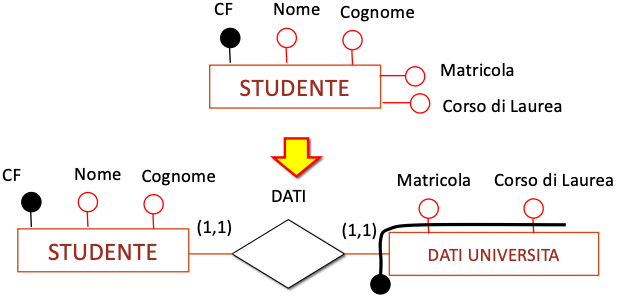
\includegraphics[width=0.5\textwidth]{foto 6.png}
\end{center}
Le operazioni che riguardano \textbf{i dati anagrafici} non riguardano \textbf{i dati dell'università}.\\
In questo caso lo schema con due entità presenta un costo inferiore rispetto allo schema con una sola entità, risultato opposto rispetto al caso precedente dell'\textit{accorpamento}.\vspace{14pt}\\
\textit{Analisi delle ridondanze}\\
Nel modello E/R, potrebbero essere presenti \textbf{ridondanze sui dati}, ossia \textbf{informazioni significative ma derivabili da altre} già presenti nel modello E/R. La ridondanza sui dati può portare a \textit{vantaggi} e \textit{svantaggi}:
\begin{itemize}[label={-}, leftmargin=1cm]
    \itemsep0em
    \item \textbf{Vantaggio}: operazioni sui dati più efficienti
    \item \textbf{Svantaggio}: maggiore occupazione di memoria
    \item \textbf{Svantaggio}: maggiore complessità degli aggiornamenti\\
\end{itemize}
Alcuni esempi di \textbf{ridondanza concettuale} in un diagramma E/R potrebbero essere:
\begin{center}
    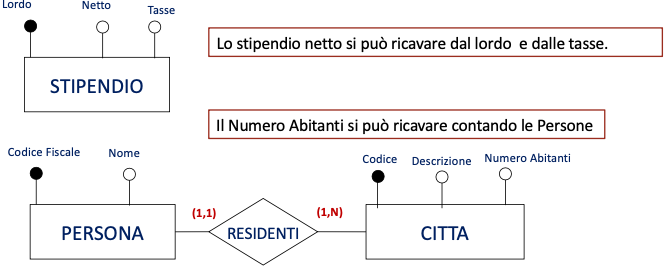
\includegraphics[width=0.65\textwidth]{foto 7.png}
\end{center}
In questa fase della progettazione logica, è necessario valutare cosa fare delle \textbf{ridondanze concettuali}.\\
Osservando l'esempio di \textit{Persona} e \textit{Città}, sono presenti due possibili soluzioni: \textbf{eliminare l'attributi} \textit{NumeroAbitanti}, o \textbf{conservare l'attributo} nel diagramma E/R.\vspace{14pt}\\
Per scegliere cosa fare di un attributo ridondante, è possibile utilizzare l'\textbf{analisi del modello E/R} visto nella progettazione concettuale.\vspace{14pt}\\
Sia \textit{S} lo schema \textbf{E/R senza ridondanze}\\
Sia \textit{$S_r$} lo schema \textbf{E/R con ridondanze}
\begin{enumerate}[leftmargin=1cm]
    \itemsep0em
    \item Si \textbf{calcolano il costo e l'occupazione di memoria} di entrambi gli schemi: \\
    \textit{<c(S), m(S)> e <c($S_r$), m($S_r$)>}
    \item Si \textbf{confrontano} \textit{c(S)/c($S_r$)} e \textit{|m(S) - m($S_r$)|}. Il rapporto dei costi viene detto \textbf{speedup}. Con un valore pari ad uno ci si trova in uno stato di indifferenza
    \item Si prende una \textbf{decisione} in base al valore delle metriche
\end{enumerate}
Inoltre, per effettuare l'analisi del modello E/R, è necessario disporre delle \textbf{tavole delle operazioni e dei volumi}.
\begin{center}
    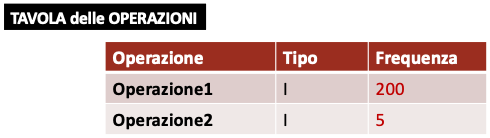
\includegraphics[width=0.45\textwidth]{foto 8.png}
\end{center}
Dove:
\begin{itemize}[label={-}, leftmargin=1cm]
    \itemsep0em
    \item \textbf{Operazione1}: inserire una nuova persona (200 volte al giorno)
    \item \textbf{Operazione2}: visualizzare tutti i dati di una città, incluso il numero di abitanti (5 volte al giorno)
\end{itemize}
\begin{center}
    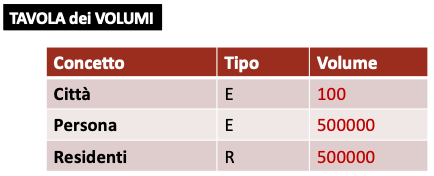
\includegraphics[width=0.45\textwidth]{foto 9.png}
\end{center}
Si inizi con l'analisi dello \textbf{schema con ridondanza \textit{$S_r$}}:\\
\begin{center}
    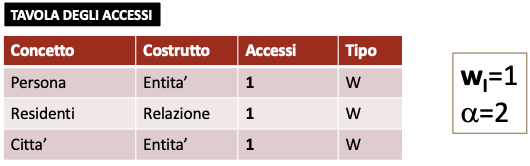
\includegraphics[width=0.5\textwidth]{foto 10.png}\vspace{10pt}\\
    \textbf{c(OP1) = 200 $\cdot$ 1 $\cdot$ (3 $\cdot$ 2) = 1200}\vspace{10pt}\\
    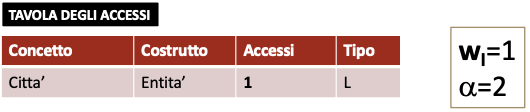
\includegraphics[width=0.5\textwidth]{foto 11.png}\vspace{10pt}\\
    \textbf{c(OP2) = 5 $\cdot$ 1 $\cdot$ (0 $\cdot$ 2 + 1) = 5}
\end{center}
Passando all'analisi dello \textbf{schema senza ridondanza \textit{S}}:\\
\begin{center}
    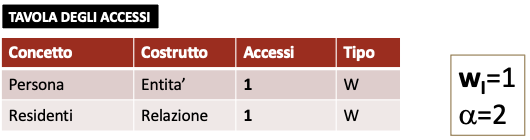
\includegraphics[width=0.5\textwidth]{foto 12.png}\vspace{10pt}\\
    \textbf{c(OP1) = 200 $\cdot$ 1 $\cdot$ (2 $\cdot$ 2) = 800}\vspace{10pt}\\
    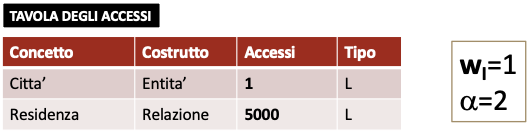
\includegraphics[width=0.5\textwidth]{foto 13.png}\vspace{10pt}\\
    \textbf{c(OP2) = 5 $\cdot$ 1 $\cdot$ (0 $\cdot$ 2 + 5001) = 25005}
\end{center}
Riassumendo:
\begin{center}
    \textbf{c($S_r$) = c(OP1) + c(OP2) = 1200 + 5 = 1205}\vspace{10pt}\\
    \textbf{c(S) = c(OP1) + c(OP2) = 800 + 25005 = 25805}\vspace{30pt}\\
\end{center}
Passando all'occupazione di memoria:
\begin{center}
    \textbf{m(S) = X byte}\vspace{10pt}\\
    \textbf{m($S_r$) = X + 100 $\cdot$ 4 = X + 400 byte}
\end{center}
Per concludere, la \textbf{presenza della ridondanza} introduce un overhead di memoria di \textbf{400 byte}, ma migliora lo speedup delle operazioni di circa \textbf{20 volte}.\\
In questo caso è conveniente \textbf{mantenere, o introdurre,} l'attributo \textit{NumeroAbitanti}.

\subsection*{Traduzione nel modello logico}
\large

La \textbf{progettazione logica} deve tradurre i costrutti del modello E/R nei costrutti del modello logico di riferimento, nel nostro caso nel \textbf{modello relazionale}, garantendo l'\textbf{equivalenza} dei modelli.\\
In sintesi, le \textbf{entità} diventano \textbf{tabelle} sugli stessi attributi, e le \textbf{relazioni del modello E/R} diventano \textbf{tabelle} sugli identificatori delle entità coinvolte (più gli attributi propri), ma sono possibili traduzioni differenti sulla base delle cardinalità.\vspace{14pt}\\
\textit{Traduzione di entità con identificatore interno}\\
\begin{center}
    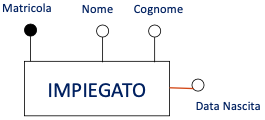
\includegraphics[width=0.3\textwidth]{foto 14.png}
\end{center}
Le entità del modello E/R si traducono in tabelle del modello relazionale. L’identificatore del modello E/R diventa la \textbf{chiave primaria} della tabella. Quindi:\\
\begin{itemize}[label={ }, leftmargin=1cm]
    \item \textbf{IMPIEGATO}(\underline{Matricola}, Nome, Cognome, DataNascita)\\
\end{itemize}
\textit{Traduzione di entità con identificatore esterno}\\
\begin{center}
    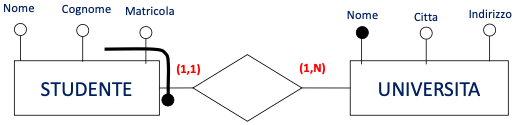
\includegraphics[width=0.5\textwidth]{foto 15.png}
\end{center}
Le entità con \textbf{identificatore esterno} si traducono in una \textbf{tabella che include tra le chiavi gli identificatori dell'entità esterna}. Quindi:
\begin{itemize}[label={ }, leftmargin=1cm]
    \item \textbf{STUDENTE}(\underline{Matricola, NomeUniversita}, Nome, Cognome)
    \item \textbf{UNIVERSITA}(\underline{Nome}, Citta, Indirizzo)\vspace{14pt}\\
\end{itemize}
\textit{Traduzione di relazioni molti a molti}\\
\begin{center}
    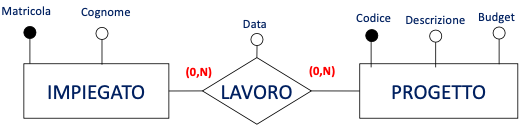
\includegraphics[width=0.5\textwidth]{foto 16.png}
\end{center}
\textbf{Ogni entità diventa una tabella} con lo stesso nome, stessi attributi e per chiave il suo identificatore.\\
\textbf{Ogni relazione diventa una tabella}, con gli stessi attributi e come chiave gli identificatori delle entità coinvolte.\\
Quindi:
\begin{itemize}[label={ }, leftmargin=1cm]
    \item \textbf{IMPIEGATO}(\underline{Matricola}, Cognome)
    \item \textbf{PROGETTO}(\underline{Codice}, Descrizione, Budget)
    \item \textbf{LAVORO}(\underline{Matricola, Codice}, Data)\\
\end{itemize}
\textit{Traduzione di relazioni uno a molti}\\
\begin{center}
    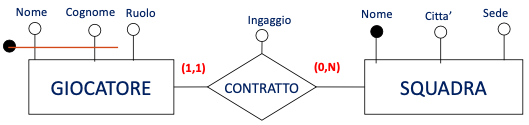
\includegraphics[width=0.5\textwidth]{foto 17.png}
\end{center}
Sono possibili \textbf{due traduzioni}:
\begin{enumerate}[leftmargin=1cm]
    \item Traducendo la \textbf{relazione come una tabella separata}, come nel caso delle relazioni molti a molti
    \item \textbf{Inglobando la relazione nell'entità} con cardinalità massima 1 (il prof. consiglia questa soluzione!)
\end{enumerate}
Si osservino le due traduzioni.\\
\textit{Traduzione 1}:
\begin{itemize}[label={ }, leftmargin=1cm]
    \item \textbf{GIOCATORE}(\underline{Nome, Cognome}, Ruolo)
    \item \textbf{SQUADRA}(\underline{Nome}, Citta, Sede)
    \item \textbf{CONTRATTO}(\underline{Nome, Cognome}, NomeSquadra, Ingaggio)
\end{itemize}
\textit{Traduzione 2}:
\begin{itemize}[label={ }, leftmargin=1cm]
    \item \textbf{GIOCATORE}(\underline{Nome, Cognome}, Ruolo, NomeSquadra, Ingaggio)
    \item \textbf{SQUADRA}(\underline{Nome}, Citta, Sede)
\end{itemize}
Cosa accade se varia la cardinalità minima di \textit{GIOCATORE}?
\begin{itemize}[label={-}, leftmargin=1cm]
    \item \textbf{cardMin = 0}: \textbf{soluzione 1} preferibile
    \item \textbf{cardMin = 1}: \textbf{soluzione 2} preferibile\\
\end{itemize}
\textit{Traduzione di relazioni uno a uno}\\
\begin{center}
    
\includegraphics[width=0.5\textwidth]{foto 18.png}
\end{center}
Sono possibili \textbf{3 diverse alternative}, in base alla \textbf{cardinalità minima} delle due entità in gioco:\vspace{14pt}\\
\textit{Caso 1}\\
Cardinalità obbligatorie per entrambe le entità (cardMin = 1 per entrambe). Si traduce il modello \textbf{inglobando la relazione in una delle due entità}.
\begin{itemize}[label={ }, leftmargin=1cm]
    \item \textbf{IMPIEGATO}(\underline{Nome, Cognome}, Stipendio, Data, NomeUfficio)
    \item \textbf{UFFICIO}(\underline{Nome}, Citta, Sede)
\end{itemize}
In alternativa, è possibile inglobare la relazione \textit{DIREZIONE} nell'entità \textit{UFFICIO}.\vspace{14pt}\\
\textit{Caso 2}\\
Partecipazione obbligatoria per una delle entità (cardMax = 1 per una delle due). Si traduce il modello \textbf{inglobando la relazione nell'entità che ha Partecipazione obbligatoria}.
\begin{itemize}[label={ }, leftmargin=1cm]
    \item \textbf{IMPIEGATO}(\underline{Nome, Cognome}, Stipendio)
    \item \textbf{UFFICIO}(\underline{Nome}, Citta, Sede, Data, NomeDirettore, CognomeDirettore)\\
\end{itemize}
\textit{Caso 3}\\
Partecipazione facoltativa per entrambe le entità (cardMin = 0 per entrambe). Si traduce il modello \textbf{traducendo la relazione come una tabella a sè stante}, come nel caso uno a molti. E' anche possibile \textbf{accorpare} (il prof. suggerisce questo!).
\begin{itemize}[label={ }, leftmargin=1cm]
    \item \textbf{IMPIEGATO}(\underline{Nome, Cognome}, Stipendio)
    \item \textbf{UFFICIO}(\underline{Nome}, Citta, Sede)
    \item \textbf{DIREZIONE}(\underline{NomeUfficio}, NomeDirettore, CognomeDirettore, Data)\vspace{100pt}\\
\end{itemize}
Come per la fase di progettazione concettuale, è necessario \textbf{corredare lo schema logico di opportuna documentazione} perchè \textbf{non tutti i vincoli sono esprimibili nello schema logico}:
\begin{itemize}[label={-}, leftmargin=1cm]
    \item Tabella delle \textbf{business rules}
    \item \textbf{Insieme dei vincoli di integrità} referenziali:
    \begin{itemize}[label={-}, leftmargin=1cm]
        \item Rappresentati \textbf{attraverso tabella}
        \item Rappresentati \textbf{in maniera grafica}, con un \textbf{diagramma logico}
        \begin{center}
            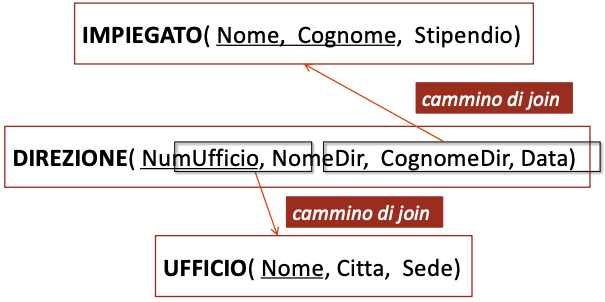
\includegraphics[width=0.5\textwidth]{foto 19.png}
        \end{center}
    \end{itemize}
\end{itemize}
\end{document}